\lab{Optimal Reentry of a Spacecraft}{Optimal Reentry of a Spacecraft}
\label{lab:reentry}
\objective{ We consider the problem of minimizing the heating experienced by a spacecraft during reentry. 
The boundary value problem (BVP) associated with the reentry of a spacecraft is inherently challenging: the craft must descend quickly enough to enter the atmosphere, but pull out soon enough to prevent overheating or crashing. 
Problems involving variational calculus and optimal control often include the numerical solution of a challenging BVP. }

\begin{figure}
\centering
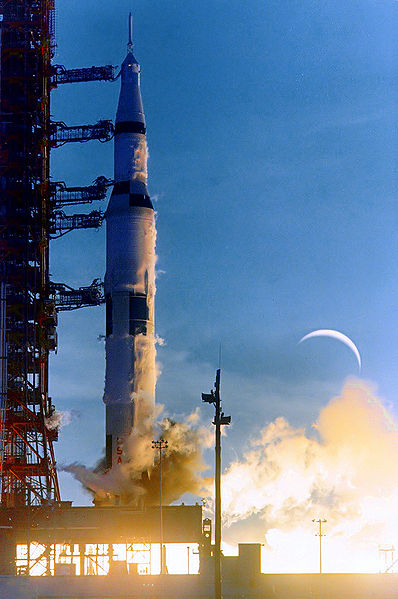
\includegraphics[width=6cm]{Apollo8_during_Launch.jpg}
\caption{Apollo 8 during launch}
\label{fig:reentry:apollo8}
\end{figure}

A fundamental topic considered in aerospace engineering is the process of landing a spacecraft. 
Landing a spacecraft requires a massive reduction in the kinetic energy of the craft. 
That reduction can be accomplished either through the use of massive quantities of fuel (very expensive), or by  transforming kinetic energy into heat. 
That heat must then be absorbed by the atmosphere and the spacecraft. 
The question then is how to choose the optimal path for reentry into the atmosphere, where the total heating experienced by the craft is minimized. 

We begin with a control system\footnote{This control problem and its numerical solution are thoroughly described in `Introduction to Numerical Analysis' by J. Stoer, R. Bulirsch (pg 524). 
We will mirror their presentation throughout this lab.}
that describes the path of a spacecraft through the atmosphere 
(we assume the spacecraft is similar to the Apollo craft).
The dependent variables are the velocity $v$ of the spacecraft,  
the angle $\gamma$ of the flight path, 
and the normalized altitude $\xi=h/R$ above the Earth's surface, where $R$ is the radius of the Earth and $h$ is the altitude of the spacecraft above the Earth.
The control variable  $u$ represents the angle of attack of the spacecraft. 
The flight path is given by 
\begin{align}
\begin{split}
\dot{v} &= -s\rho v^2C_D(u) - \frac{g\sin(\gamma)}{(1+\xi)^2},\\
\dot{\gamma} &= s \rho v C_L(u) + \frac{v \cos(\gamma)}{R(1+\xi)} - \frac{g \cos \gamma}{v(1+\xi)^2},\\
\dot{\xi} &= \frac{v \sin \gamma}{R}.
\end{split} \label{eqn:reentry:control_system}
\end{align}
Coefficients $C_D$ and $C_L$ represent drag and lift coefficients, and depend on the angle of attack:
\begin{align*}
 C_D(u) &= 1.174 - .9\cos u, \\
 C_L(u) &= 0.6\sin u.
\end{align*}
 
The atmospheric density $\rho$ is a function of height,
\[\rho(\xi) = \rho_0e^{-R\beta\xi},
\] where  $\rho_0$ is the atmospheric density at the surface of the earth. 
Other parameters include the force of gravity $g$, and $s = \frac{1}{2}S/m$, where $S$ is the frontal area of the craft and $m$ is its mass.
The numerical values we will use are coded below, along with the drag and lift functions. 
\begin{lstlisting}
from __future__ import division
from math import pi, sqrt, sin, cos, exp
from numpy import linspace, array, tanh, cosh, ones, arctan
import numpy as np
from scipy.special import erf
from scipy.optimize import root

from bvp6c import bvp6c, bvpinit, deval
from structure_variable import struct

R = 209
beta = 4.26
rho0 = 2.704e-3
g = 3.2172e-4
s = 26600

def C_d(u):
	return 1.174 - 0.9*cos(u)

def C_l(u):
	return 0.6*sin(u)
\end{lstlisting}

Realistic boundary conditions for the trajectory of the spacecraft are
\begin{equation}
  \begin{split}
    v(0) &= 0.36 \quad (36000 \text{ ft/sec})\\
    \gamma(0) &= -8.1^\circ \frac{\pi}{180^\circ}\\
    \xi(0)&= \frac{4}{R}\quad (h = 400000 \text{ ft})
  \end{split} 
\quad \quad \quad \quad \quad
  \begin{split}
    v(T) &= 0.27\\
    \gamma(T) &= 0 \\
	\xi(T)&= \frac{2.5}{R}
  \end{split} \label{eqn:reentry:BCs}
\end{equation}
where $T$ represents the time at the end of the (first) reentry maneuver. 
These boundary conditions are similar to those encountered at the end of each Apollo mission to the moon. 

% To simpify notation, we will also write \eqref{eqn:reentry:control_system} in the form $y' = G(y)$, where $y = [y_0, y_1, y_2]^T=[v,\gamma, \xi]^T$ and $G$ has component functions $G = [G_0, G_1, G_2]^T$.
The total heating is 
\[
J[u] = \int_0^T 10 v^3 \sqrt{\rho}.
\]
The Hamiltonian corresponding to this control system\footnote{Here we are using the Pontryagin Minimum Principle, rather than the Maximum Principle. Due to this slight variation, the Hamiltonian is defined as  $\lambda  \cdot f + L$, where $\lambda$ is the costate vector, the state equation is $\dot{x} = f,$ and the functional $J = \int_0^T L$.} is 
\begin{align}
	\begin{split}
H &=  10v^3 \sqrt{\rho} + \lambda_1 \left ( -s\rho v^2C_D(u) - \frac{g\sin(\gamma)}{(1+\xi)^2} \right) + \\ 
&{ }\quad \quad\lambda_2 \left( s \rho v C_L(u) + \frac{v \cos(\gamma)}{R(1+\xi)} - \frac{g \cos \gamma}{v(1+\xi)^2} \right) + \\
&{ }\quad \quad \lambda_3 \left( \frac{v \sin \gamma}{R} \right),
	\end{split}
\end{align}
% \begin{align}
% H &=  10y_0^3 \sqrt{\rho} + \lambda_0G_0 + \lambda_1G_1 + \lambda_2G_2,
% \end{align}
where $\lambda = [\lambda_1,\lambda_2,\lambda_3]^T$ is the adjoint variable. 
The state and adjoint equations are thus given by 
\begin{align}
\begin{split}
	\dot{y} &= H_{\lambda},\quad \dot{} = \frac{d}{dt},\\
	\dot{\lambda} &= -H_{y}, \label{eqn:reentry:full_system}
\end{split}
\end{align}
where $y = [y_1,y_2,y_3]^T = [v,\gamma, \xi]^T$.
To our boundary conditions we add the terminal condition that $H = 0$ at $t = T$. 
Finally, from the condition $\frac{\partial H}{\partial u} = 0$ we find that the optimal control satisfies 
\begin{align}
\tan u &= \frac{6\lambda_2}{9v\lambda_1}.
\end{align}

Most BVP solvers require an equal number of differential equations and boundary conditions. 
Currently we have a free boundary value problem; there are 6 ODEs and 7 boundary conditions, and the length of the reentry maneuver, $T$, is still unknown. 
By making the transformation $x = t/T$, and treating $T$ as a dependent variable, the BVP is now defined on the interval $(0,1)$ and is augmented with an additional ODE: 
\begin{align}
\begin{split}
	y' &= TH_{\lambda},\quad ' = \frac{d}{dx},\\
	\lambda' &= -TH_{y},\\
	T' &= 0. \label{eqn:reentry:full_system}
\end{split}	
\end{align}
This BVP has 7 ODEs, and with the 7 boundary conditions introduced earlier it has the required form.
% \footnote{BNDSCO - A program for the numerical solution of optimal control problems, H.J. Oberle and W. Grimm, 1989}


\begin{figure}
\centering
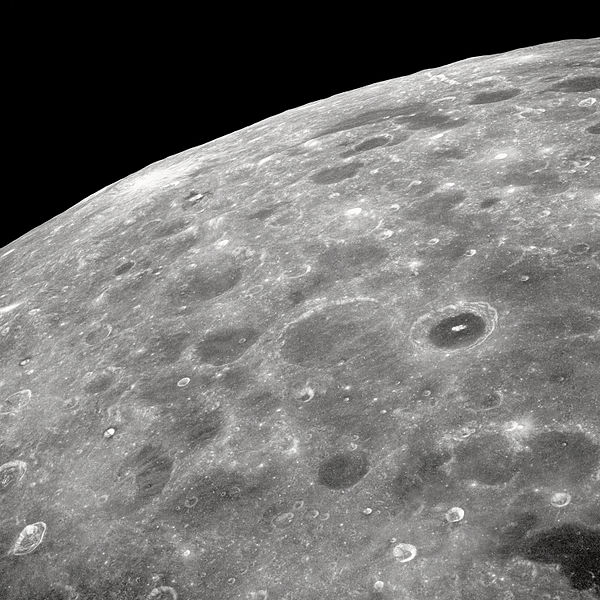
\includegraphics[width=7cm]{The_Lunar_Farside.jpg}
\caption{ The Apollo 8 mission was the first to orbit the moon and return to earth. 
After a flight of three days from earth, they orbited the moon ten times in 20 hours before making the return trip. 
This photograph  shows a portion of the far side of the moon, as seen by the Apollo 8.
}
\label{fig:reentry:Lunar_Farside}
\end{figure}



\begin{problem}
Complete the function \li{ode} below that implements the right hand side of \eqref{eqn:reentry:full_system}. 
Notice that the adjoint variables and the final time are coordinates of $y:$ $y_4 = \lambda_1$, $y_5 = \lambda_2$, $y_6=\lambda_3$, and $y_7 = T$. Finally, note that we use Python zero based indexing below.
\begin{lstlisting}
def ode(x,y):
	# Parameters:
	# x: independent variable (unused in our ODEs)
	# y: vector-valued dependent variable; it is an ndarray 
	# 	 with shape (7,)
	
	# Returns: 
	# ndarray of length (7,) that evalutes the RHS of the ODES
	u =	 arctan((6*y[4])/(9*y[0]*y[3] ))
	rho = rho0*exp(-beta*R*y[2])
	out = y[6]*array([
				 # G_0
				 -s*rho*y[0]**2*C_d(u) - g*sin(y[1])/(1+y[2])**2,	
				 # G_1	 
				( s*rho*y[0]*C_l(u) + y[0]*cos(y[1])/(R*(1 + y[2])) - 
				  g*cos(y[1])/(y[0]*(1+y[2])**2) ),						 
				 # G_2
				y[0]*sin(y[1])/R,		
				 # G_3								 
				-( 30*y[0]**2.*sqrt(rho)+ y[3]*(-2*s*rho*y[0]*C_d(u)) + 
				   y[4]*( s*rho*C_l(u) +cos(y[1])/(R*(1 + y[2])) + 
						  g*cos(y[1])/( y[0]**2*(1+y[2])**2 ) 
							) + 
				   y[5]*(sin(y[1])/R)	   ),	
				  # G_4						 
				-( y[3]*( -g*cos(y[1])/(1+y[2])**2	) + 
				   y[4]*( -y[0]*sin(y[1])/(R*(1+y[2])) + 
						  g*sin(y[1])/(y[0]*(1+y[2])**2 ) 
							) + 
				   y[5]*(y[0]*cos(y[1])/R )	   ),
				  # G_5 -- This line needs to be completed.						 
				  ,			
				  # G_6	
					0 									 
			   ])
	return out
\end{lstlisting}
\end{problem}

\begin{figure}
\centering
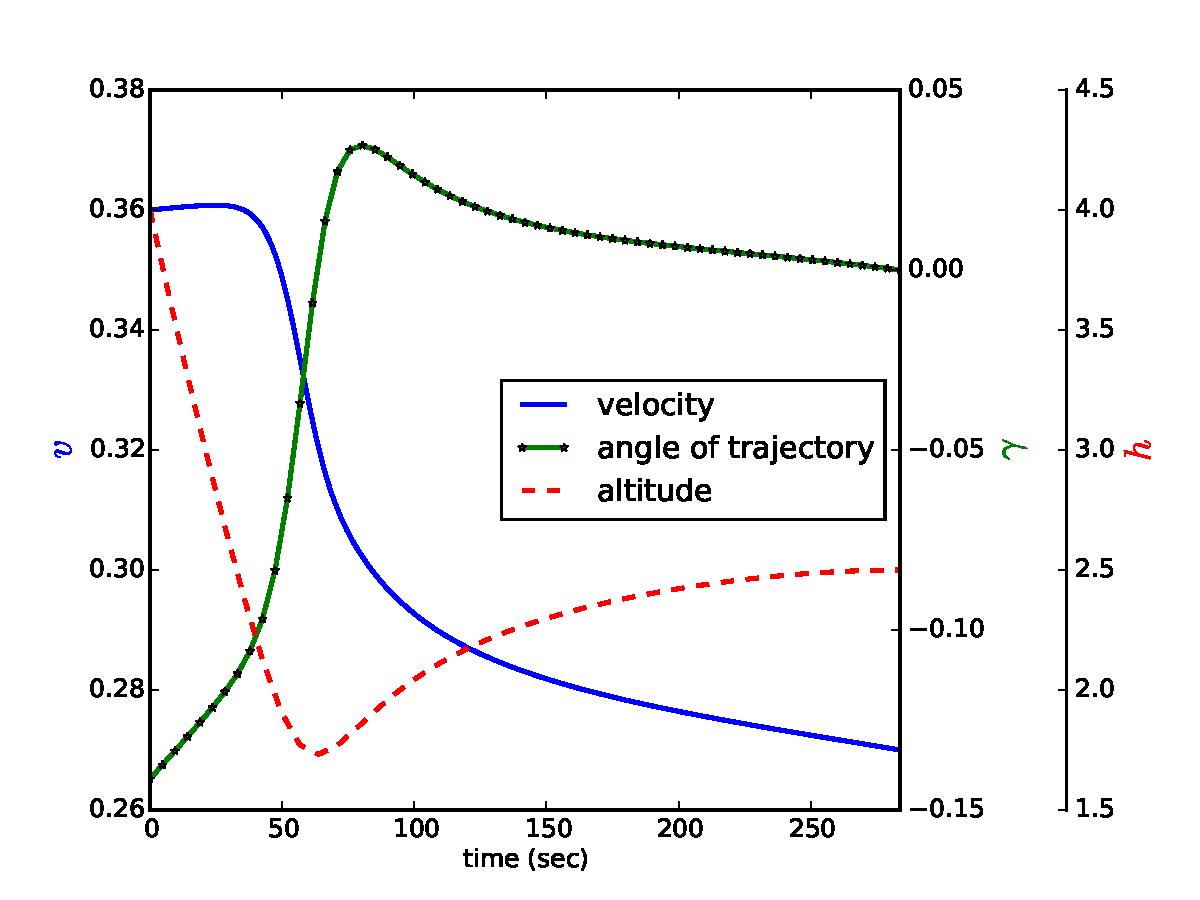
\includegraphics[width=\textwidth]{solutions.pdf}
\caption{The optimal path for the reentry maneuver of a spacecraft. 
This path minimizes the heating of the spacecraft, and satisfies  \eqref{eqn:reentry:full_system},\eqref{eqn:reentry:BCs}, and the terminal condition $H(T) = 0$.
}
\label{fig:reentry:solutions}
\end{figure}


\section*{Constructing an Initial Guess}
We will use the BVP solver \li{scikits.bvp_solver}.
Like any solver capable of handling nonlinear problems, \li{bvp_solver} requires an initial guess to jump-start its Newton-like iteration process.
% We will use the BVP solver \li{bvp6c}. 
% Like any solver capable of handling nonlinear problems, \li{bvp6c} requires an initial guess to jump-start its Newton-like iteration process.
Our nonlinear BVP is very sensitive, and requires an initial guess that is quite close to the solution.  
This sensitivity is physically meaningful. 
The spacecraft is traveling at a speed far greater than a typical aircraft. 
If the control is not aggressive, the spacecraft will fall/`bounce' back into space as it encounters the atmosphere at a high velocity. 
However, if the control lasts too long, the craft will overheat or crash.

Since this is a sensitive problem, we will use a heuristic method to construct good initial guesses for $v, \gamma, \xi, \lambda_1, \lambda_2,\lambda_2$, and $u$.
From aerospace engineers we know that the control $u$ should empirically look like Figure \ref{fig:reentry:estimate_u}; 
we can create a smooth approximation of the form $u = p_1\erf(p_2(p_3-t/T))$, where $p_1, p_2,$ and $p_3$ are unknown constants. 
To help us determine these constants, and to find good initial guesses for $v, \gamma$, and $\xi$, we define an auxiliary BVP
\begin{align}
\begin{split}
\dot{y_0} &= -s\rho y_0^2C_D(u) - \frac{g\sin(y_1)}{(1+y_2)^2},\\
\dot{y_1} &= s \rho y_0 C_L(u) + \frac{y_0 \cos(y_1)}{R(1+y_2)} - \frac{g \cos y_1}{y_0(1+y_2)^2},\\
\dot{y_2} &= \frac{y_0 \sin y_1}{R} ,\\
\dot{p_1} &= 0, \\
\dot{p_2} &= 0, \\
\dot{p_3} &= 0.
\end{split} \label{eqn:reentry:control_system_auxiliary}
\end{align}

This auxiliary BVP is defined on the interval $[0,T]$, where $T$ is unknown. 
We guess at $T$: the maneuver will occur quickly, so how about 230 seconds?  After this boundary value problem has been solved, we will have good initial guesses for the correct $v,\gamma,\xi$, and $u.$ We will still need to construct initial guesses for $\lambda_1, \lambda_2$, and $\lambda_3$.
Below we code  functions for \eqref{eqn:reentry:control_system_auxiliary} and for the boundary conditions. 
\begin{lstlisting}
T0 = 230	
	
def ode_auxiliary(t,y):
	u = y[3]*erf( y[4]*(y[5]-(1.*t)/T0) )
	rho = rho0*exp(-beta*R*y[2])
	out = array([-s*rho*y[0]**2*C_d(u) - g*sin(y[1])/(1+y[2])**2,
				  ( s*rho*y[0]*C_l(u) + y[0]*cos(y[1])/(R*(1 + y[2])) -
				  g*cos(y[1])/(y[0]*(1+y[2])**2) ),
				  y[0]*sin(y[1])/R,
				  0,
				  0,
				  0		])
	return out

def bcs_auxiliary(ya,yb):
	out1 = array([ ya[0]-.36,
				  ya[1]+8.1*pi/180,
				  ya[2]-4/R
				  ])
	out2 = array([ yb[0]-.27,
				  yb[1],
				  yb[2]-2.5/R
				  ])
	return out1, out2
\end{lstlisting}

% The two main functions used by \li{bvp6c} are \li{bvpinit} and \li{deval}.
The two main functions used are \li{ProblemDefinition} and \li{solve}.
% You will want to look at their docstrings to learn more about their functionality.
The function \li{solve} requires an initial guess, which you will create in Problem \ref{prob:reentry:guess}. 

% \begin{lstlisting}
%
% options = struct()
% # options include abstol, reltol, singularterm, stats, vectorized, maxnewpts,slopeout,xint
% options.abstol, options.reltol = 1e-8, 1e-7
% options.fjacobian = ode_auxiliary_jacobian
% options.bcjacobian = bcs_auxiliary_jacobian
% options.nmax = 2000
%
% solinit = bvpinit(np.linspace(0,1,100),initial_guess)
% sol = bvp6c(ode,bcs,solinit,options)
%
% N = 240
% xint = linspace(0,T0,N+1)
% num_sol_auxiliary, _ = deval(sol,xint)
%
%
% \end{lstlisting}

\begin{lstlisting}
problem_auxiliary = bvp_solver.ProblemDefinition(num_ODE = 6,
										  num_parameters = 0,
										  num_left_boundary_conditions = 3,
										  boundary_points = (0, T0),
										  function = ode_auxiliary,
										  boundary_conditions = bcs_auxiliary)

solution_auxiliary = bvp_solver.solve(problem_auxiliary,
								solution_guess = guess_auxiliary)

N = 240
t_guess = linspace(0,T0,N+1)
guess = solution_auxiliary(t_guess)
\end{lstlisting}







\begin{figure}
\begin{minipage}[b]{.47\linewidth}
\centering
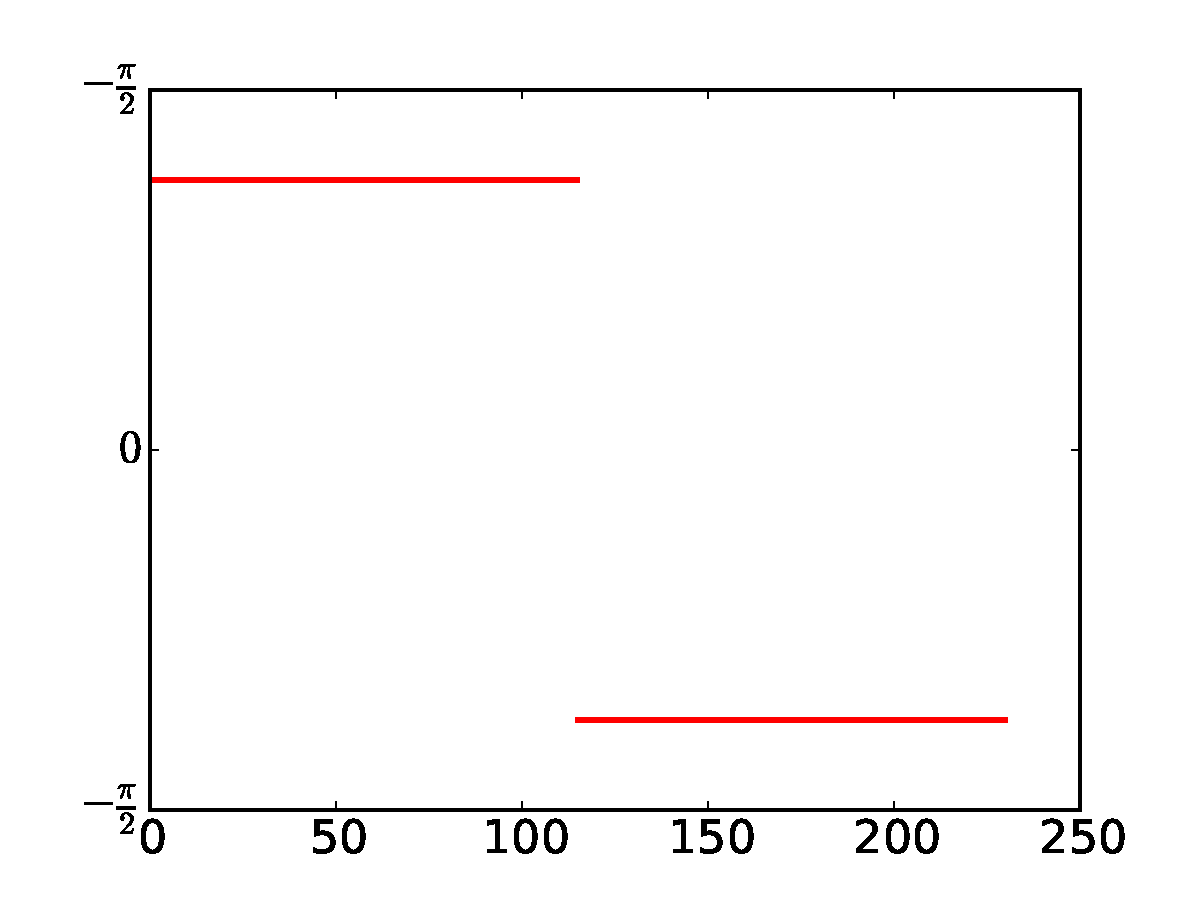
\includegraphics[width=\textwidth]{u_heuristic.pdf}
\caption*{Heuristic for the control $u$, provided by engineers. }
\end{minipage}
\hspace{0.5cm}
\begin{minipage}[b]{0.47\linewidth}
\centering
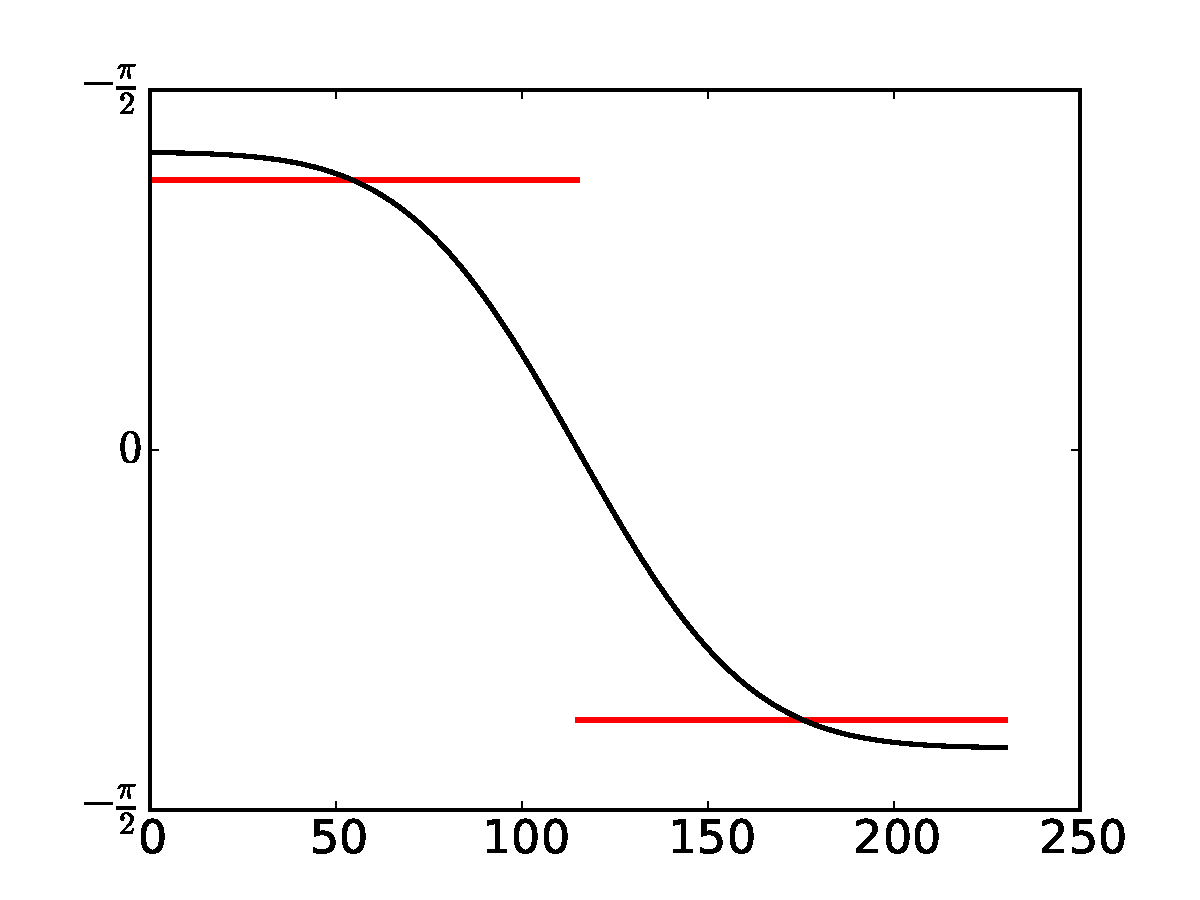
\includegraphics[width=\textwidth]{u_heuristic_smooth.pdf}
\caption*{A smooth initial approximation of the control.}
\end{minipage}
\caption{We construct a smooth estimate for the control $u$, by supposing the control has the form 
$u = p_1\erf(p_2(p_3-t/T))$ and estimating parameters $p_1, p_2, p_3$.}
\label{fig:reentry:estimate_u}
\end{figure}


\begin{problem}
	Complete the function \li{guess_auxiliary} given below. Then run the code above to check that your initial guess is adequate. 
	This function provides an initial guess to \li{bvp_solver} for the auxiliary BVP described by  \eqref{eqn:reentry:control_system_auxiliary} and \eqref{eqn:reentry:BCs}.
	Use the heuristic data provided in Figure \ref{fig:reentry:estimate_u} to find good estimates of $p_1, p_2,$ and $p_3$. 
	Use Figure \ref{fig:reentry:solutions} to estimate the trajectories of $y_1, y_2,$ and $y_3$. Hint: Try using the $\tanh$ function.
	
\begin{lstlisting}
def guess_auxiliary(t):
	out = array([ .5*(.36+.27)-.5*(.36-.27)*tanh(.025*(t-.45*T_init)),
			# Finish this line, 
			# And this one, 
			p1*ones(t.shape),
			p2*ones(t.shape),
			p3*ones(t.shape)   ])
	return out
\end{lstlisting}	
	\label{prob:reentry:guess}
\end{problem}

At this point we have constructed good initial guesses for the dependent variables $y_1,y_2, y_3,$ and $y_7$ (representing the total time of the manuever) in the original BVP \eqref{eqn:reentry:full_system}. 
We now need to construct initial guesses for the adjoint variables $y_4, y_5,$ and $y_6$. 

By reexamining the condition $H_u = 0$, we find that the optimal control $u$ satisfies 
\[
\sin u = \frac{-0.6 y_5}{\alpha} \qquad \cos u  = \frac{-0.9 y_1y_4}{\alpha}
\]
where $\alpha = \sqrt{(0.6y_5)^2 + (0.9y_1y_4)^2}$.
From this we know that $y_4 <0$, since $\cos u >0$. A simple guess would be $y_4 = -1$. 
(Recall that the adjoint variables are unique up to some scaling.) 
We can then approximate $y_5$ from the relationship 
\begin{align*}
\tan u &= \frac{6y_5}{9y_1y_4}.
\end{align*}
To approximate $y_6$, we use the identity $H = 0$.


\begin{problem}
	Adapt your previous code to solve the original, dimension seven BVP. 
	Use the solution of the auxiliary BVP to construct a good initial guess.
	Plot the control $u$. How long does the reentry maneuver take? 
\end{problem}

